\chapter{Reinforcement Learning on Mountain car}

There are various RL algorithms. Here we'll focus on Q learning, sarsa and DQN.\\
\begin{figure}[H]
    \centering
    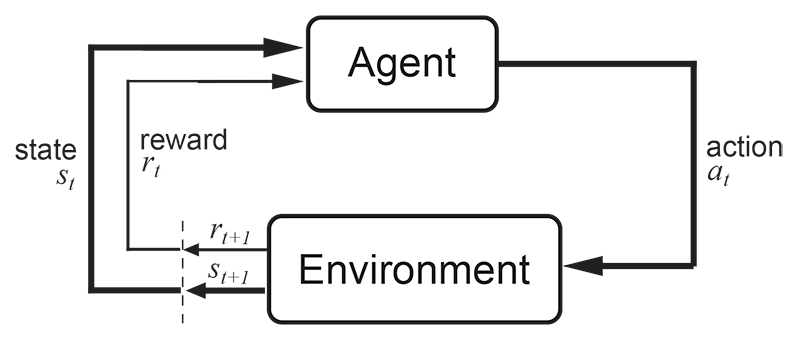
\includegraphics[width=0.8\textwidth]{images/qlearn.png}
    \caption{Agent and environment}
\end{figure}\\



\section{Q-learning}
Lets see Q learnning first.
\subsection{Algorithm}
\newline \textbf{Pseudo code}
\begin{figure}[H]
    \centering
    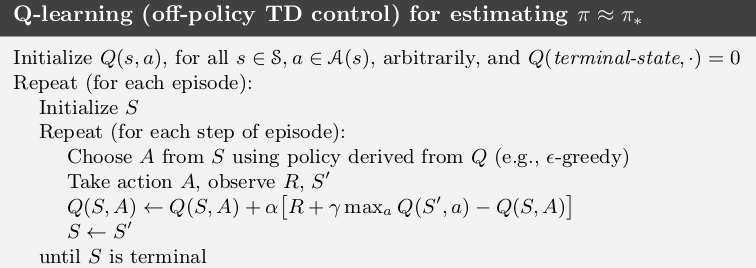
\includegraphics[width=\textwidth]{images/qlearnpseudo.png}
    % \caption{Mountain Car}
\end{figure}


\subsection{Implementation}
Openai gym is open source library for implementing the RL algorithm.\cite{openai}
Let train the mountain car using the q learning as below pseudo code. Full code of the same can be found \href{https://github.com/iamrajee/Slam_and_RL_BTP/tree/master/code/AI/mountainCar/qlearn}{here}.
\begin{figure}[H]
    \centering
    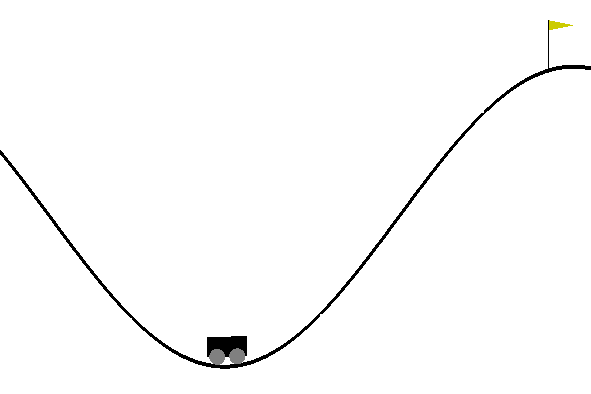
\includegraphics[width=0.5\textwidth]{images/mountaincar.png}
    \caption{Mountain Car}
\end{figure}


\textbf{Pseudo Code}
\begin{minted}{python}

def Qlearning(environment, learningRate, gamma, epsilon, n_Episodes):
    find_Number_state_in_x_and_y()
    initialise qTable and epsilon decay rate
    Run for n_Episodes
        state= resetEnvironment();
        state = discretiseState(initState)
        while not done
            action = epsilonGreedy() 
            newstate, Reward, done, info = env.step(action) 
            s_d = discret(s_)# Discretize
            update_qTable()  #as below
            '''
            Q[sd[0], sd[1],a] =(1-lr)*Q[sd[0],sd[1],a]  +   lr*(R + gamma*np.max(Q[s_d[0], s_d[1]]))
            '''
            state=newstate
        epsilionDecayUpdate()
        printAvgRper100episodes()
    env.close()
    return

\end{minted}\\

\newline \begin{figure}[H]
    \centering
    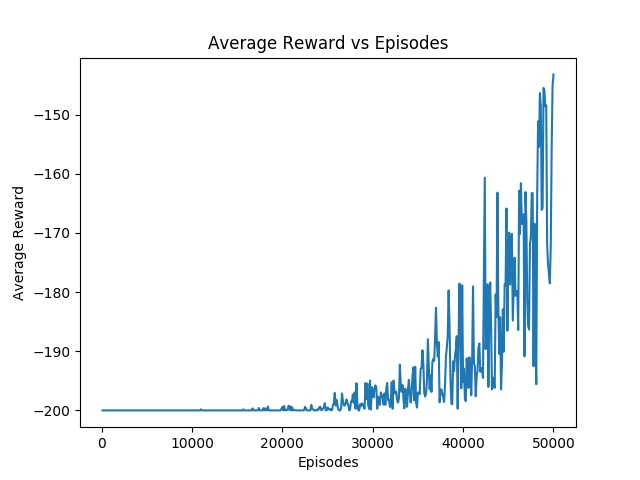
\includegraphics[width=0.8\textwidth]{images/qlearnBest.jpg}
    \caption{Result - average reward for 100 episodes}
\end{figure}\\




\newline \section{Sarsa}\\
Here we try to improve the result of above implementation by using sarsa. Fully detailed code of the same can be found \href{https://github.com/iamrajee/Slam_and_RL_BTP/tree/master/code/AI/mountainCar/sarsa}{here}.
\newline \subsection{Algorithm}\\
\begin{figure}[H]
    \centering
    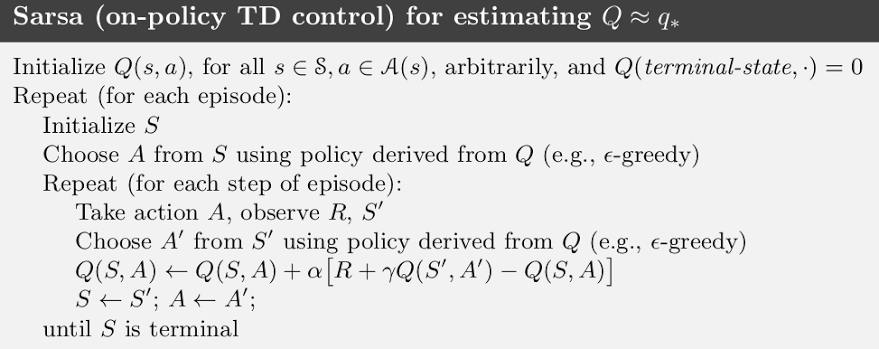
\includegraphics[width=\textwidth]{images/sarsa.png}
    % \caption{Sarsa algorithms}
\end{figure}\\

\subsection{Implementation}\\
\\
\textbf{Pseudo Code}
\begin{minted}{python}

def Sarsa(environment, learningRate, gamma, epsilon, n_Episodes):
    find_Number_state_in_x_and_y()
    initialise qTable and epsilon decay rate
    Run for n_Episodes
        state= resetEnvironment();
        state = discretiseState(initState)
        while not done
            action = epsilonGreedy() 
            newstate, Reward, done, info = env.step(action) 
            s_d = discret(s_)# Discretize
            update_qTable() #as below
            '''
            if np.random.random() < 1 - ep:#epsilon greedy exr vs expt
                    a_ = np.argmax(Q[s_d[0], s_d[1]])
                else:
                    a_ = np.random.randint(0, env.action_space.n)
            Q[sd[0], sd[1],a] =(1-lr)*Q[sd[0],sd[1],a]  +   lr*(R + gamma*Q[s_d[0], s_d[1],a_])
            '''
            state=newstate
        epsilionDecayUpdate()
        printAvgRper100episodes()
    env.close()
    return
\end{minted}\\

\newline \begin{figure}[H]
    \centering
    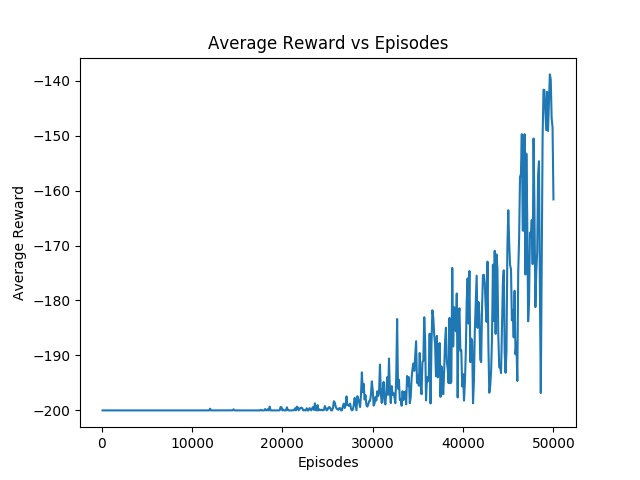
\includegraphics[width=0.8\textwidth]{images/sarsaBest.jpg}
    \caption{Result - average reward for 100 episodes}
\end{figure}\\





\newline \section{Deep Q-Network (DQN)}
\begin{figure}[H]
    \centering
    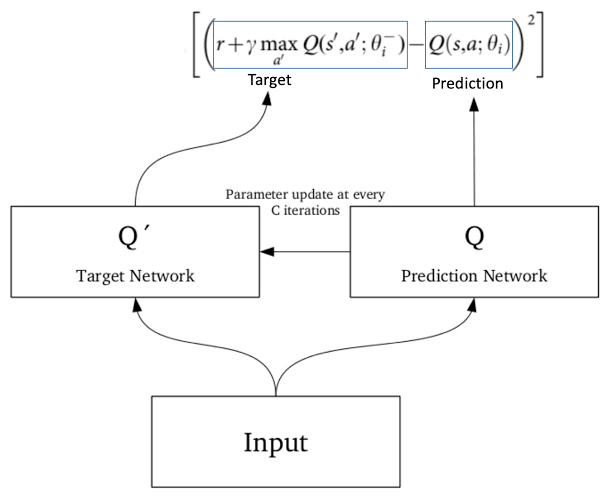
\includegraphics[width=\textwidth]{images/dqn.png}
    \caption{Flow chart of DQN}
\end{figure}\\

\newline \subsection{Algorithm}
\begin{figure}[H]
    \centering
    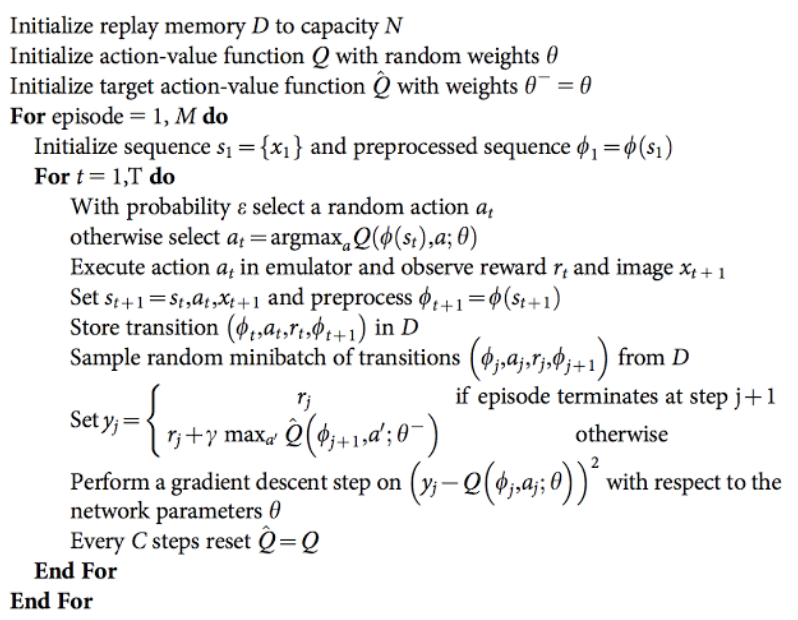
\includegraphics[width=\textwidth]{images/dqnAlgo2.png}
    \caption{Deep Q-Network algorithm}
\end{figure}


\subsection{Implementation}
I used the the keras and gym to implement DQN on mountain Car problem. Detailed code for the same can be found \href{https://github.com/iamrajee/Slam_and_RL_BTP/tree/master/code/AI/mountainCar/dqn}{here}.
\begin{figure}[H]
    \centering
    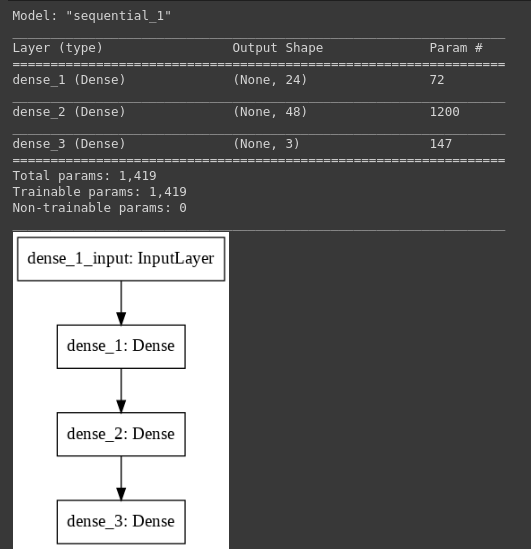
\includegraphics[width=0.8\textwidth]{images/dqnmodel1.png}
    \caption{DQN model 1(keras)}
\end{figure}
\begin{figure}[H]
    \centering
    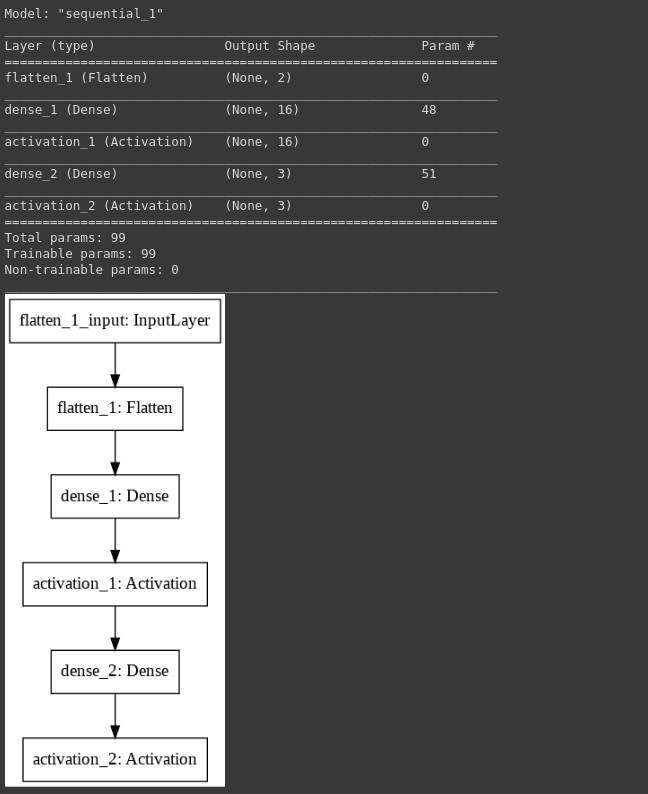
\includegraphics[width=0.8\textwidth]{images/dqnmodel2.png}
    \caption{DQN model 2(keras-rl)}
\end{figure}


\newline \section{Conclusion}
In this chapter, we studied and implemented various algorithms like Q-learning, Sarsa, DQN on the mountain car problem using the openai gym library. Here DQN out performs both q learning and sarsa which in turn out perform q learning. Average reward for q-learning is (-143), Sarsa is (-132) and DQN is (-110).
